\documentclass[12pt]{article} 
 \usepackage[pdftex]{graphicx} 
 \setlength{\paperwidth}{210mm} 
 
                                         \setlength{\paperheight}{297mm}%% 
 \usepackage{a4}%% 
 \textwidth=16cm%% 
 \textheight=23cm%% 
 
                                         \oddsidemargin=0.0cm%% 
 \evensidemargin=0.0cm%% 
 \parindent=0mm 
 \begin{document} 
%% Automatically generated Matrix Output 
\begin{center} 
 \section{Trading Grid} 
 \par 
 \begin{scriptsize} 
 \begin{tabular}{p{15.0 mm}|p{15.0 mm}|p{15.0 mm}|p{15.0 mm}|p{15.0 mm}|p{15.0 mm}|p{15.0 mm}} 
          & $\frac{S_t}{S_0}$ & $\Delta r$ & $\Delta \nu$ &     Type &    Value &    $w_k$ \\ \hline 
1 & 0.70& 0.00& 0.00& pi& 9'833.10& 1.00\\ 
2 & 0.80& 0.00& 0.00& pi& 8'109.50& 1.00\\ 
3 & 0.90& 0.00& 0.00& pi& 6'714.80& 0.50\\ 
4 & 1.00& 0.00& 0.00& delta& 8'709.10& 0.00\\ 
5 & 1.00& 0.00& 0.00& gamma& 7.41& 0.00\\ 
6 & 1.00& 0.00& 0.00& pi& 5'671.40& 10'000.00\\ 
7 & 1.00& 0.00& 0.00& rho& 281'190.00& 0.00\\ 
8 & 1.00& 0.00& 0.00& vega& 28'024.00& 0.00\\ 
9 & 1.10& 0.00& 0.00& pi& 4'945.00& 0.50\\ 
10 & 1.20& 0.00& 0.00& pi& 4'476.30& 1.00\\ 
11 & 1.30& 0.00& 0.00& pi& 4'194.90& 1.00\\ 
\end{tabular} 
  \end{scriptsize} 
 \end{center}
\section{Optimizer Task} 
 \begin{verbatim} 
 Requested Portfolio 
 -------------------- 
 -- Key Value --> Value ('Value', None, None, 250.0) 
 -- Key P1 --> Value ('P', [1, 2], [0.5, 0.6], [0, 200]) 
 -- Key P2 --> Value ('P', [4, 5], [0.5, 0.6], [0, 200]) 
 -- Key P3 --> Value ('P', [9, 10], [0.5, 0.6], [0, 200]) 
 -- Key P4 --> Value ('P', [1, 2], [0.8, 0.9], [0, 200]) 
 -- Key P5 --> Value ('P', [4, 5], [0.8, 0.9], [0, 200]) 
 -- Key P6 --> Value ('P', [9, 10], [0.8, 0.9], [0, 200]) 
 -- Key C7 --> Value ('C', [1, 1.2], [1.2, 1.4], [-2, 2]) 
 -- Key C8 --> Value ('C', [4, 4.2], [1.2, 1.4], [-2, 2]) 
 -- Key C9 --> Value ('C', [9, 9.2], [1.2, 1.4], [-2, 2]) 
 -- Key B10 --> Value ('B', None, None, [0, 250]) 
 
 
 Optimizer Result
================== 
       fun: 17825.796490489498
 hess_inv: <28x28 LbfgsInvHessProduct with dtype=float64>
      jac: array([ 1.90356224e+03,  6.03827099e+04,  5.50742652e+02, -3.39157852e+02,
        3.76050344e+04,  6.89774549e+02, -7.87875550e+02, -7.53324344e+03,
        2.03990932e+02, -3.16056418e+04, -1.68787765e+05,  3.99037784e+03,
       -3.72672987e+03, -3.47118084e+04,  8.56708726e+02, -7.55659067e+01,
       -2.50178781e+03, -1.72133296e+03, -4.60322847e+03,  6.43211064e+04,
       -1.21424132e+04,  5.17563315e+03, -6.67653345e+04, -2.14673333e+04,
        3.85493627e+03, -6.74576164e+04, -3.50401783e+04, -6.05883492e+01])
  message: 'CONVERGENCE: REL_REDUCTION_OF_F_<=_FACTR*EPSMCH'
     nfev: 14500
      nit: 356
     njev: 500
   status: 0
  success: True
        x: array([ 1.8920582 ,  0.5       ,  8.02518829,  4.11209765,  0.5       ,
        8.1067062 ,  9.00000071,  0.5       ,  6.62732308,  1.18792324,
        0.89961855, 13.27681595,  4.02478685,  0.81851319,  4.62542591,
        9.00000007,  0.80428979,  0.2013064 ,  1.00000388,  1.26741195,
        1.69469003,  4.19999945,  1.26309058, -1.89482338,  9.00913283,
        1.20012115, -1.89982887,  9.4283859 ])
 \end{verbatim}
%% Automatically generated Matrix Output 
\begin{center} 
 \section{Asset Directory} 
 \par 
 \begin{scriptsize} 
 \begin{tabular}{p{17.5 mm}|p{17.5 mm}|p{17.5 mm}|p{17.5 mm}|p{17.5 mm}|p{17.5 mm}} 
          &     Type &      $t$ &    $S_t$ &   Strike &   Number \\ \hline 
1 & B& 0.00& None& None& 9.42\\ 
2 & C& 1.00& 1'289.10& 1'633.80& 1.69\\ 
3 & C& 4.20& 1'289.10& 1'628.20& -1.89\\ 
4 & C& 9.00& 1'289.10& 1'547.10& -1.89\\ 
5 & P& 1.18& 1'289.10& 1'159.70& 13.27\\ 
6 & P& 1.89& 1'289.10& 644.54& 8.02\\ 
7 & P& 4.02& 1'289.10& 1'055.10& 4.62\\ 
8 & P& 4.11& 1'289.10& 644.54& 8.10\\ 
9 & P& 9.00& 1'289.10& 1'036.80& 0.20\\ 
10 & P& 9.00& 1'289.10& 644.54& 6.62\\ 
\end{tabular} 
  \end{scriptsize} 
 \end{center}%% Automatically generated Matrix Output 
\begin{center} 
 \section{Valuation} 
 \par 
 \begin{scriptsize} 
 \begin{tabular}{p{17.5 mm}|p{17.5 mm}|p{17.5 mm}|p{17.5 mm}|p{17.5 mm}|p{17.5 mm}} 
          &    $\pi$ & $\delta$ & $\gamma$ &   $\rho$ &    $\nu$ \\ \hline 
  1.30 & -1'286.10& -4'258.00& 6.72& -22'506.00& 1'144.00\\ 
  1.20 & -917.83& -5'006.30& 10.83& -23'326.00& 3'119.40\\ 
  1.10 & -431.04& -6'258.60& 16.37& -25'168.00& 5'595.60\\ 
  1.00 & 250.00& -8'102.70& 22.85& -28'408.00& 8'289.90\\ 
  0.90 & 1'226.60& -10'456.00& 28.44& -33'300.00& 10'574.00\\ 
  0.80 & 2'608.00& -12'918.00& 30.38& -39'787.00& 11'771.00\\ 
  0.70 & 4'473.80& -14'844.00& 27.87& -47'537.00& 11'909.00\\ 
\end{tabular} 
  \end{scriptsize} 
 \end{center}%% Automatically generated Matrix Output 
\begin{center} 
 \subsection{Valuation Details at level 1.30} 
 \par 
 \begin{scriptsize} 
 \begin{tabular}{p{13.1 mm}|p{13.1 mm}|p{13.1 mm}|p{13.1 mm}|p{13.1 mm}|p{13.1 mm}|p{13.1 mm}|p{13.1 mm}} 
          &     Type &      $t$ &    $S_t$ &   Strike &    $\pi$ & $\delta$ &   $\rho$ \\ \hline 
1 & B& 0.00& None& None& 9.42& 0.00& 0.00\\ 
2 & C& 1.00& 1'289.10& 1'633.80& 297.48& 1'788.60& 1'491.10\\ 
3 & C& 4.20& 1'289.10& 1'628.20& -696.58& -2'188.60& -6'266.30\\ 
4 & C& 9.00& 1'289.10& 1'547.10& -1'121.80& -2'464.60& -12'098.00\\ 
5 & P& 1.18& 1'289.10& 1'159.70& 63.78& -678.19& -881.42\\ 
6 & P& 1.89& 1'289.10& 644.54& 0.11& -1.60& -3.26\\ 
7 & P& 4.02& 1'289.10& 1'055.10& 100.75& -477.92& -2'329.00\\ 
8 & P& 4.11& 1'289.10& 644.54& 6.36& -44.45& -209.00\\ 
9 & P& 9.00& 1'289.10& 1'036.80& 9.94& -27.09& -333.31\\ 
10 & P& 9.00& 1'289.10& 644.54& 44.46& -164.14& -1'877.50\\ 
\end{tabular} 
  \end{scriptsize} 
 \end{center}%% Automatically generated Matrix Output 
\begin{center} 
 \subsection{Valuation Details at level 1.20} 
 \par 
 \begin{scriptsize} 
 \begin{tabular}{p{13.1 mm}|p{13.1 mm}|p{13.1 mm}|p{13.1 mm}|p{13.1 mm}|p{13.1 mm}|p{13.1 mm}|p{13.1 mm}} 
          &     Type &      $t$ &    $S_t$ &   Strike &    $\pi$ & $\delta$ &   $\rho$ \\ \hline 
1 & B& 0.00& None& None& 9.42& 0.00& 0.00\\ 
2 & C& 1.00& 1'289.10& 1'633.80& 176.28& 1'248.90& 1'072.60\\ 
3 & C& 4.20& 1'289.10& 1'628.20& -536.57& -1'814.70& -5'368.00\\ 
4 & C& 9.00& 1'289.10& 1'547.10& -937.12& -2'154.70& -10'969.00\\ 
5 & P& 1.18& 1'289.10& 1'159.70& 142.01& -1'331.30& -1'750.10\\ 
6 & P& 1.89& 1'289.10& 644.54& 0.33& -4.33& -8.84\\ 
7 & P& 4.02& 1'289.10& 1'055.10& 145.20& -637.43& -3'149.90\\ 
8 & P& 4.11& 1'289.10& 644.54& 10.96& -72.21& -342.02\\ 
9 & P& 9.00& 1'289.10& 1'036.80& 12.29& -31.61& -395.17\\ 
10 & P& 9.00& 1'289.10& 644.54& 59.34& -209.01& -2'415.20\\ 
\end{tabular} 
  \end{scriptsize} 
 \end{center}%% Automatically generated Matrix Output 
\begin{center} 
 \subsection{Valuation Details at level 1.10} 
 \par 
 \begin{scriptsize} 
 \begin{tabular}{p{13.1 mm}|p{13.1 mm}|p{13.1 mm}|p{13.1 mm}|p{13.1 mm}|p{13.1 mm}|p{13.1 mm}|p{13.1 mm}} 
          &     Type &      $t$ &    $S_t$ &   Strike &    $\pi$ & $\delta$ &   $\rho$ \\ \hline 
1 & B& 0.00& None& None& 9.42& 0.00& 0.00\\ 
2 & C& 1.00& 1'289.10& 1'633.80& 89.99& 755.34& 665.35\\ 
3 & C& 4.20& 1'289.10& 1'628.20& -395.01& -1'446.20& -4'415.00\\ 
4 & C& 9.00& 1'289.10& 1'547.10& -763.33& -1'844.70& -9'742.10\\ 
5 & P& 1.18& 1'289.10& 1'159.70& 303.23& -2'448.60& -3'269.00\\ 
6 & P& 1.89& 1'289.10& 644.54& 0.98& -11.72& -24.04\\ 
7 & P& 4.02& 1'289.10& 1'055.10& 209.31& -841.00& -4'227.20\\ 
8 & P& 4.11& 1'289.10& 644.54& 19.09& -117.75& -562.73\\ 
9 & P& 9.00& 1'289.10& 1'036.80& 15.26& -36.80& -468.66\\ 
10 & P& 9.00& 1'289.10& 644.54& 79.99& -267.21& -3'124.80\\ 
\end{tabular} 
  \end{scriptsize} 
 \end{center}%% Automatically generated Matrix Output 
\begin{center} 
 \subsection{Valuation Details at level 1.00} 
 \par 
 \begin{scriptsize} 
 \begin{tabular}{p{13.1 mm}|p{13.1 mm}|p{13.1 mm}|p{13.1 mm}|p{13.1 mm}|p{13.1 mm}|p{13.1 mm}|p{13.1 mm}} 
          &     Type &      $t$ &    $S_t$ &   Strike &    $\pi$ & $\delta$ &   $\rho$ \\ \hline 
1 & B& 0.00& None& None& 9.42& 0.00& 0.00\\ 
2 & C& 1.00& 1'289.10& 1'633.80& 37.54& 374.49& 336.95\\ 
3 & C& 4.20& 1'289.10& 1'628.20& -274.40& -1'094.20& -3'443.00\\ 
4 & C& 9.00& 1'289.10& 1'547.10& -602.42& -1'537.60& -8'425.20\\ 
5 & P& 1.18& 1'289.10& 1'159.70& 614.03& -4'143.70& -5'651.90\\ 
6 & P& 1.89& 1'289.10& 644.54& 2.91& -31.44& -65.01\\ 
7 & P& 4.02& 1'289.10& 1'055.10& 301.26& -1'092.60& -5'609.90\\ 
8 & P& 4.11& 1'289.10& 644.54& 33.63& -192.26& -928.90\\ 
9 & P& 9.00& 1'289.10& 1'036.80& 19.05& -42.66& -555.50\\ 
10 & P& 9.00& 1'289.10& 644.54& 108.96& -342.71& -4'065.10\\ 
\end{tabular} 
  \end{scriptsize} 
 \end{center}%% Automatically generated Matrix Output 
\begin{center} 
 \subsection{Valuation Details at level 0.90} 
 \par 
 \begin{scriptsize} 
 \begin{tabular}{p{13.1 mm}|p{13.1 mm}|p{13.1 mm}|p{13.1 mm}|p{13.1 mm}|p{13.1 mm}|p{13.1 mm}|p{13.1 mm}} 
          &     Type &      $t$ &    $S_t$ &   Strike &    $\pi$ & $\delta$ &   $\rho$ \\ \hline 
1 & B& 0.00& None& None& 9.42& 0.00& 0.00\\ 
2 & C& 1.00& 1'289.10& 1'633.80& 11.89& 141.17& 129.28\\ 
3 & C& 4.20& 1'289.10& 1'628.20& -176.70& -772.43& -2'502.10\\ 
4 & C& 9.00& 1'289.10& 1'547.10& -456.58& -1'237.70& -7'037.50\\ 
5 & P& 1.18& 1'289.10& 1'159.70& 1'164.20& -6'312.90& -8'882.20\\ 
6 & P& 1.89& 1'289.10& 644.54& 8.56& -82.85& -172.96\\ 
7 & P& 4.02& 1'289.10& 1'055.10& 431.92& -1'389.10& -7'329.10\\ 
8 & P& 4.11& 1'289.10& 644.54& 59.86& -313.05& -1'533.40\\ 
9 & P& 9.00& 1'289.10& 1'036.80& 23.89& -49.13& -657.23\\ 
10 & P& 9.00& 1'289.10& 644.54& 150.09& -440.41& -5'314.50\\ 
\end{tabular} 
  \end{scriptsize} 
 \end{center}%% Automatically generated Matrix Output 
\begin{center} 
 \subsection{Valuation Details at level 0.80} 
 \par 
 \begin{scriptsize} 
 \begin{tabular}{p{13.1 mm}|p{13.1 mm}|p{13.1 mm}|p{13.1 mm}|p{13.1 mm}|p{13.1 mm}|p{13.1 mm}|p{13.1 mm}} 
          &     Type &      $t$ &    $S_t$ &   Strike &    $\pi$ & $\delta$ &   $\rho$ \\ \hline 
1 & B& 0.00& None& None& 9.42& 0.00& 0.00\\ 
2 & C& 1.00& 1'289.10& 1'633.80& 2.57& 36.39& 33.81\\ 
3 & C& 4.20& 1'289.10& 1'628.20& -102.82& -496.33& -1'652.70\\ 
4 & C& 9.00& 1'289.10& 1'547.10& -328.17& -951.08& -5'611.80\\ 
5 & P& 1.18& 1'289.10& 1'159.70& 2'040.50& -8'456.10& -12'469.00\\ 
6 & P& 1.89& 1'289.10& 644.54& 24.90& -210.73& -445.84\\ 
7 & P& 4.02& 1'289.10& 1'055.10& 614.88& -1'713.60& -9'371.50\\ 
8 & P& 4.11& 1'289.10& 644.54& 107.42& -505.14& -2'518.90\\ 
9 & P& 9.00& 1'289.10& 1'036.80& 30.08& -55.99& -774.78\\ 
10 & P& 9.00& 1'289.10& 644.54& 209.19& -565.87& -6'975.60\\ 
\end{tabular} 
  \end{scriptsize} 
 \end{center}%% Automatically generated Matrix Output 
\begin{center} 
 \subsection{Valuation Details at level 0.70} 
 \par 
 \begin{scriptsize} 
 \begin{tabular}{p{13.1 mm}|p{13.1 mm}|p{13.1 mm}|p{13.1 mm}|p{13.1 mm}|p{13.1 mm}|p{13.1 mm}|p{13.1 mm}} 
          &     Type &      $t$ &    $S_t$ &   Strike &    $\pi$ & $\delta$ &   $\rho$ \\ \hline 
1 & B& 0.00& None& None& 9.42& 0.00& 0.00\\ 
2 & C& 1.00& 1'289.10& 1'633.80& 0.32& 5.48& 5.16\\ 
3 & C& 4.20& 1'289.10& 1'628.20& -52.05& -279.71& -956.16\\ 
4 & C& 9.00& 1'289.10& 1'547.10& -219.58& -685.61& -4'198.50\\ 
5 & P& 1.18& 1'289.10& 1'159.70& 3'272.70& -9'765.20& -15'488.00\\ 
6 & P& 1.89& 1'289.10& 644.54& 70.55& -504.23& -1'087.50\\ 
7 & P& 4.02& 1'289.10& 1'055.10& 865.54& -2'027.30& -11'643.00\\ 
8 & P& 4.11& 1'289.10& 644.54& 193.67& -799.87& -4'085.50\\ 
9 & P& 9.00& 1'289.10& 1'036.80& 38.03& -62.83& -907.79\\ 
10 & P& 9.00& 1'289.10& 644.54& 295.18& -724.35& -9'175.70\\ 
\end{tabular} 
  \end{scriptsize} 
 \end{center}\begin{figure} 
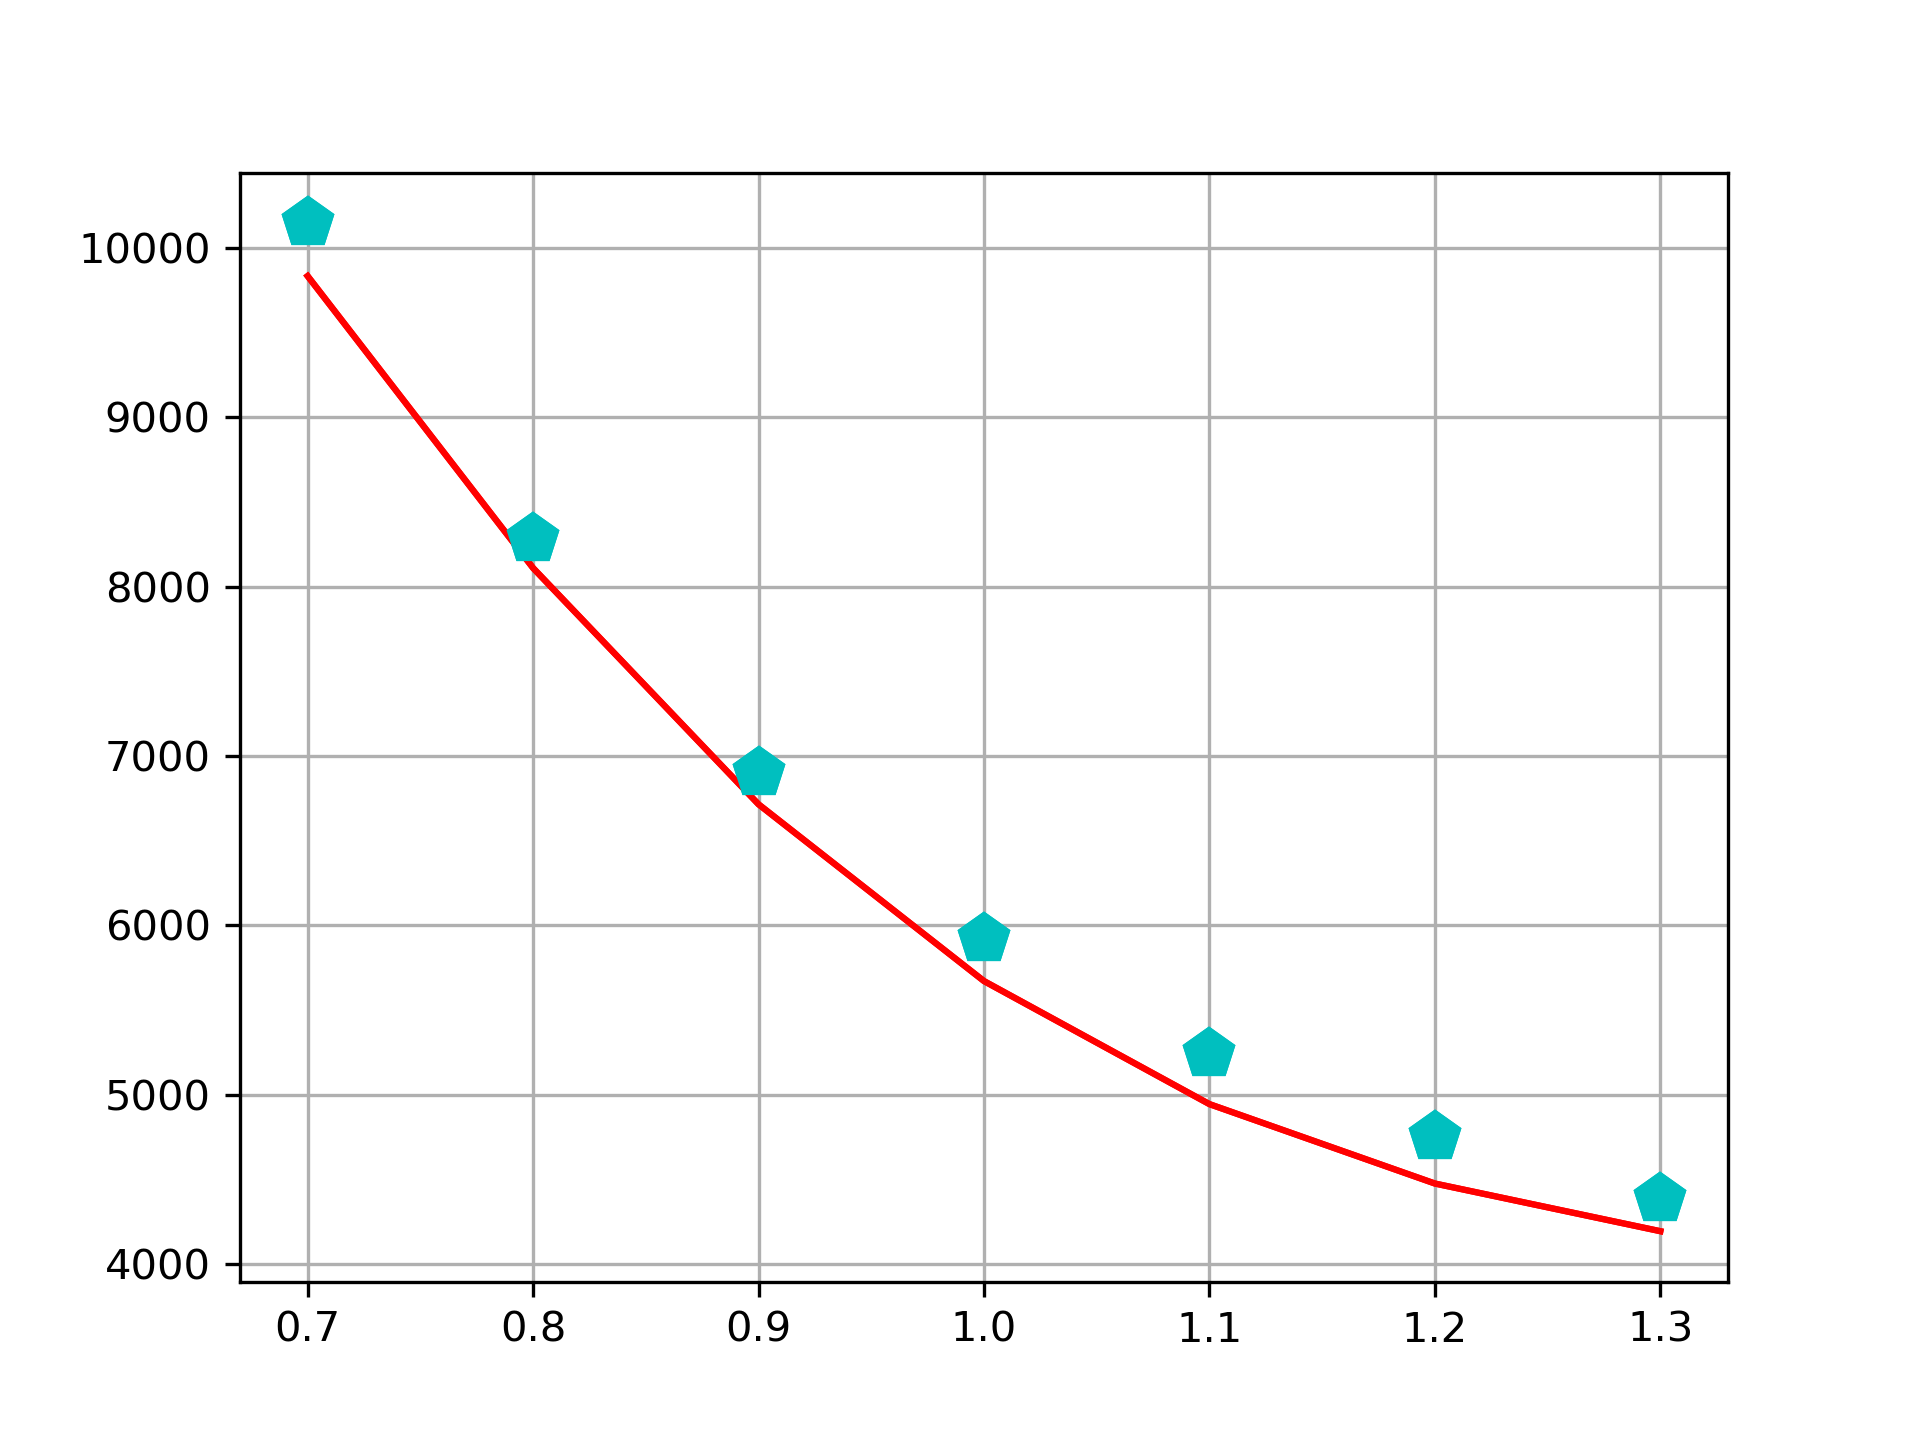
\includegraphics[width=0.9\textwidth]{task40.png} 
\caption{Adjusted Comparision} 
 \end{figure}\begin{figure} 
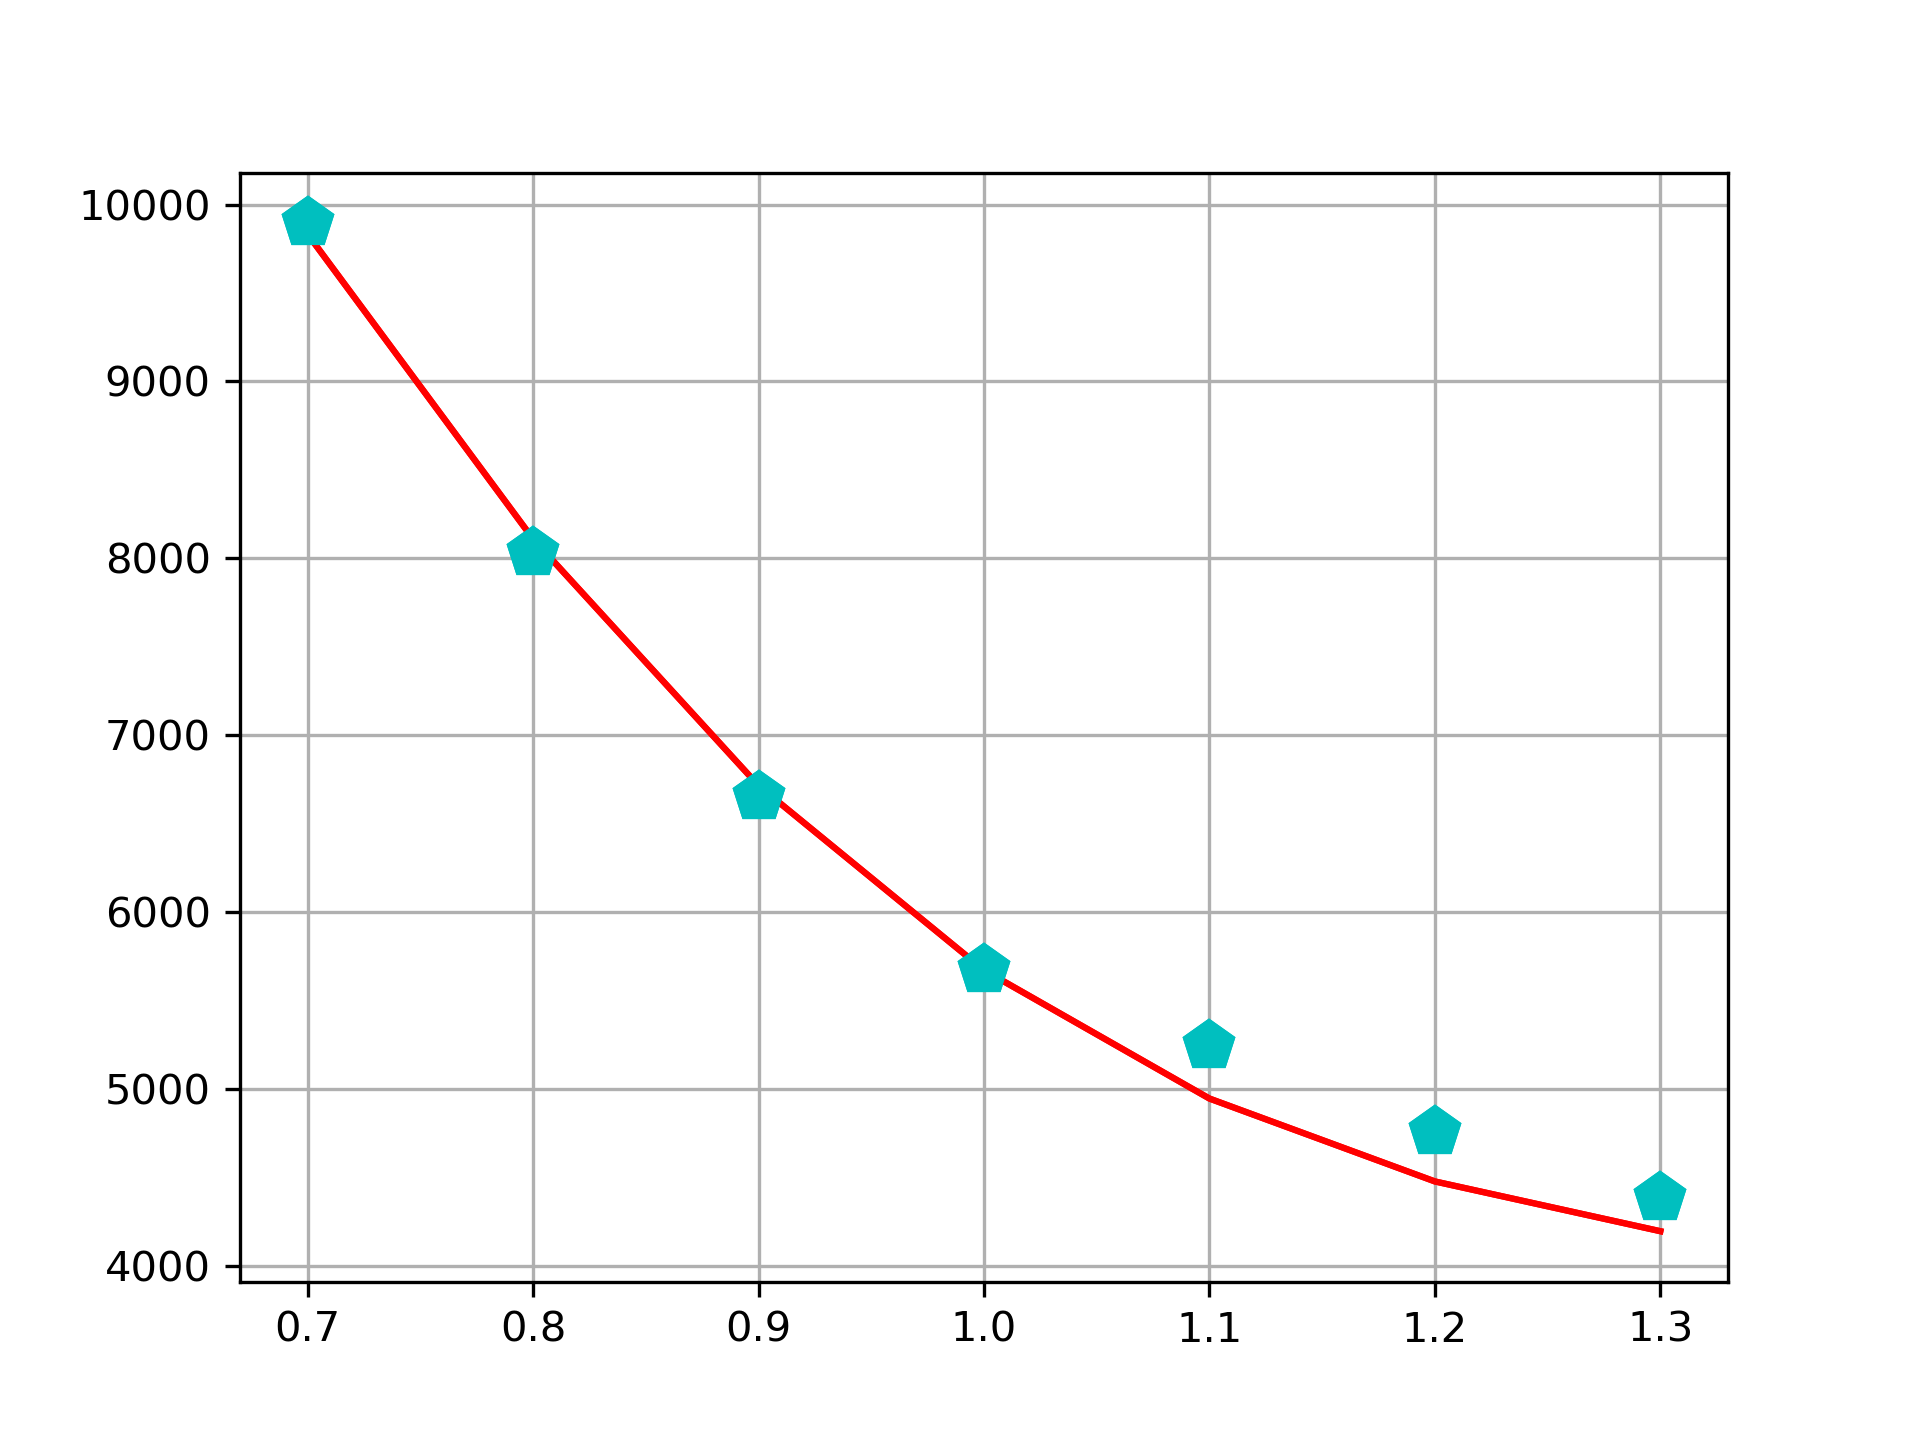
\includegraphics[width=0.9\textwidth]{task41.png} 
\caption{Adjusted Comparision} 
 \end{figure}\begin{figure} 
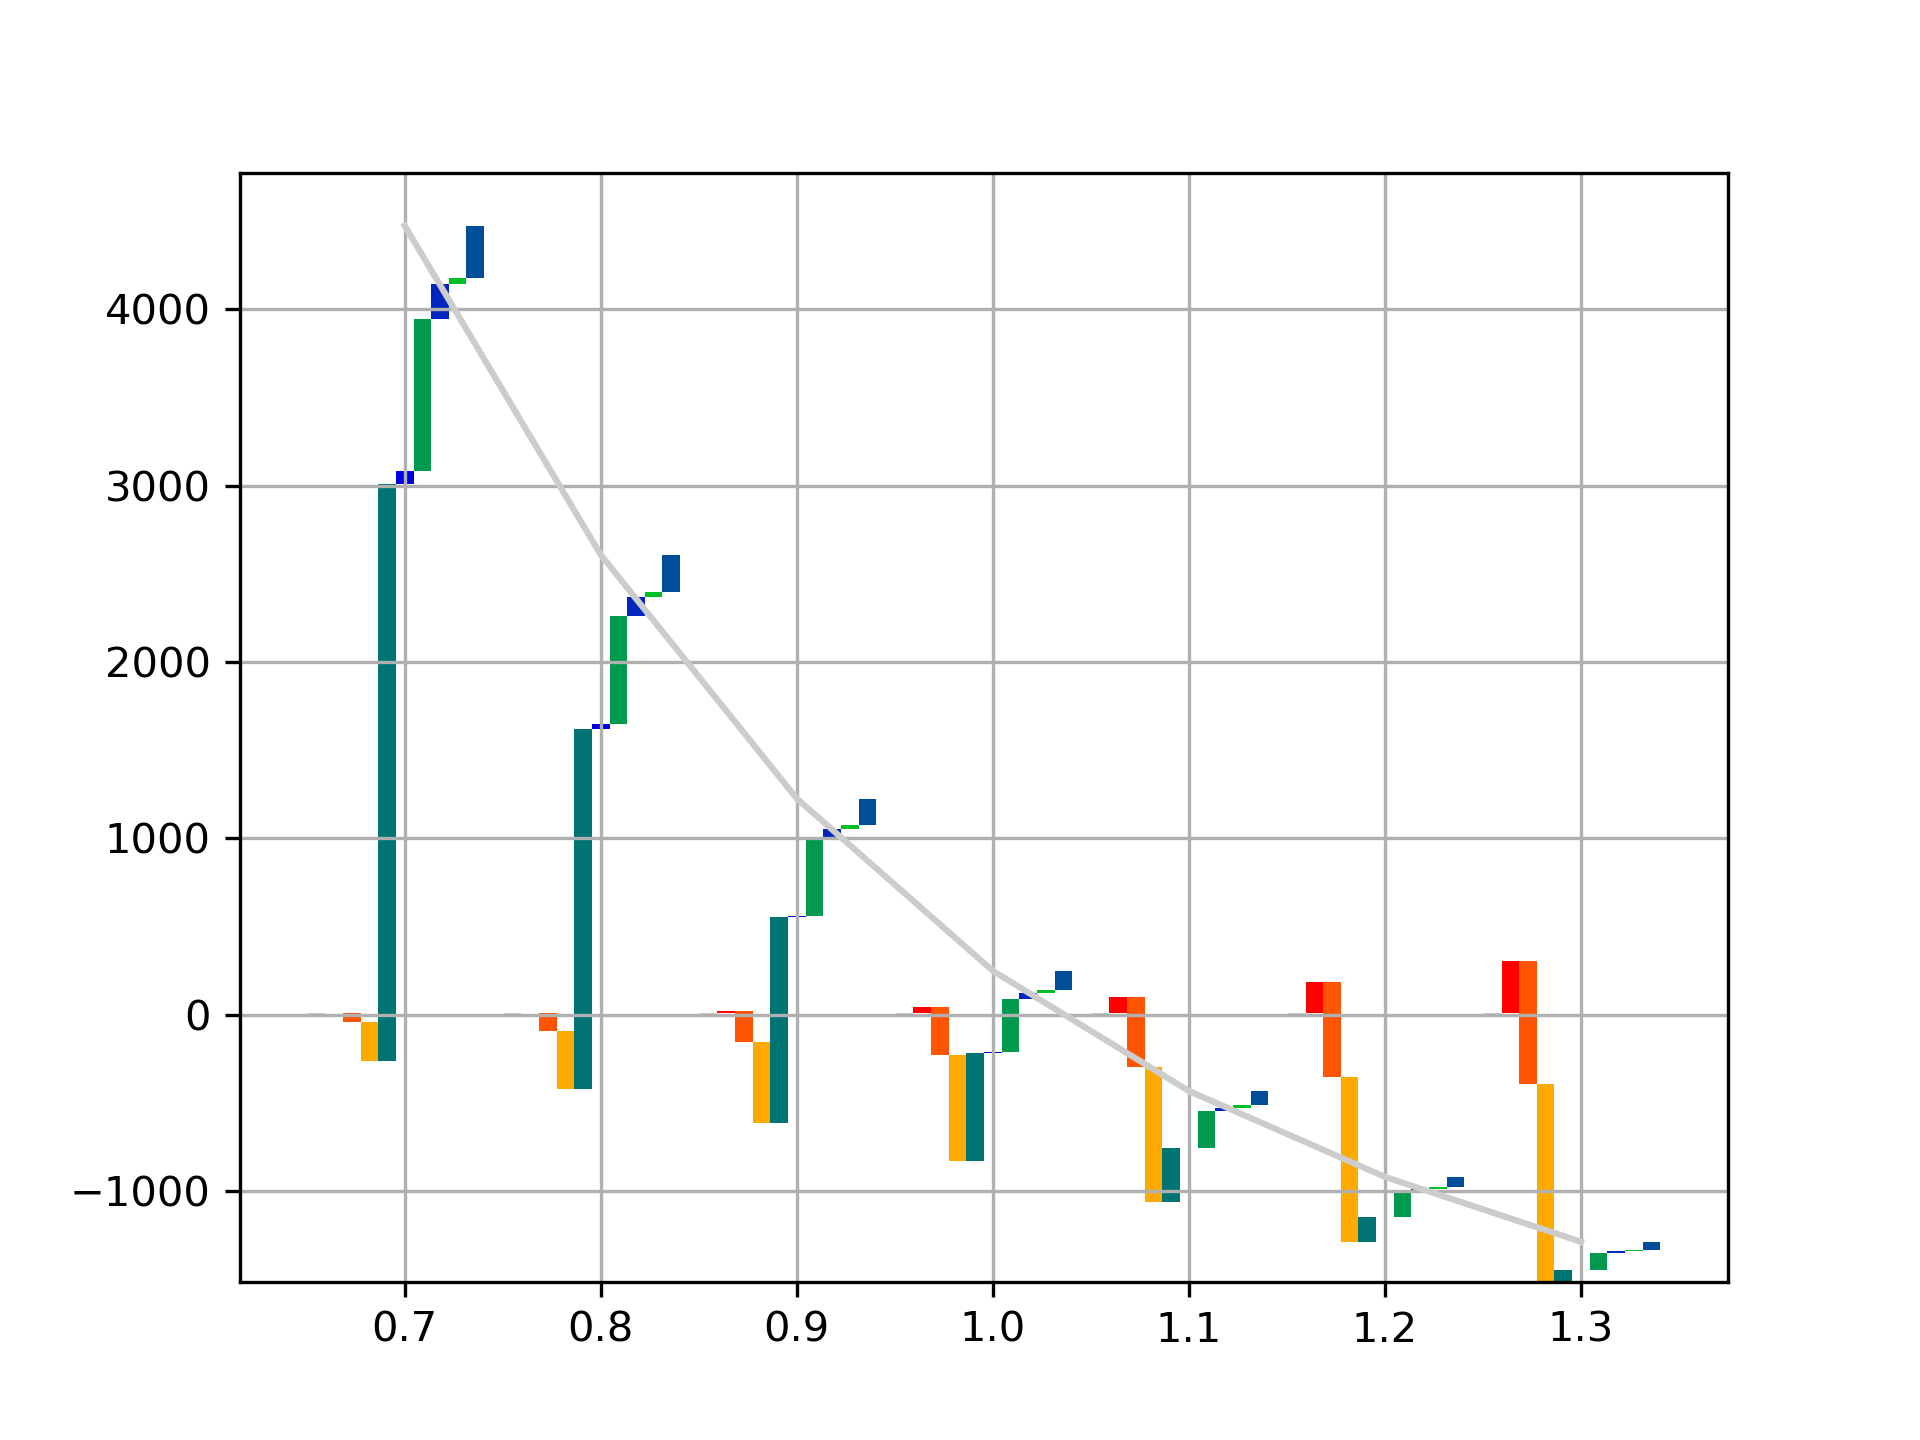
\includegraphics[width=0.9\textwidth]{task42.png} 
\caption{Decomposition P\&L} 
 \end{figure}
\end{document}